
\documentclass[10pt,oneside,letterpaper,colorhighlight]{book}


\def\pdfBorderAttrs{/Border [0 0 0] } % No border around Links
%\usepackage{thumbpdf}
%\pdfcompresslevel=9



\usepackage{alltt}
\usepackage{cite}
\usepackage{plain}
\usepackage{hyperref}
\usepackage{varioref}
\usepackage{array}
\usepackage{xypic}
\usepackage{color}
\usepackage{sectsty}
\usepackage{fancyhdr}
\usepackage{graphics}
\usepackage{fancyvrb}
\usepackage{listings}
\usepackage{makeidx}
\usepackage[nottoc]{tocbibind}

\usepackage [dvips] {graphicx}
\usepackage{wrapfig}


\hypersetup{
    backref,  
	colorlinks,
    pdftitle={Drools Usage Manual},
    pdfsubject={Drools Usage Manual},
    pdfkeywords={Drools, Rules, Rete, Java},
    pdfauthor={The Drools Project}} 
\makeindex

\fancypagestyle{plain}{
    \fancyhf{}
    \fancyfoot[C]{\usefont{OT1}{phv}{b}{n}\selectfont \thepage }
    \renewcommand{\footrulewidth}{0pt}
    \renewcommand{\headrulewidth}{0pt}
}

\pagestyle{fancy}

\fancyhf{}
\fancyhead[L]{ \usefont{OT1}{phv}{b}{n}\selectfont \small \leftmark}
\fancyhead[R]{ \usefont{OT1}{phv}{b}{n}\selectfont \small \rightmark }
\fancyfoot[C]{\usefont{OT1}{phv}{b}{n}\selectfont \thepage }
\renewcommand{\footrulewidth}{0pt}
\renewcommand{\headrulewidth}{0.5pt}

\renewcommand{\chaptermark}[1]{%
	\markboth{#1}{}}

\renewcommand{\sectionmark}[1]{%
	\markright{#1\ : \thesection}}

\allsectionsfont{\usefont{OT1}{phv}{b}{n}\selectfont}

%%%%%%
%%%%%%

%\renewcommand{\theFancyVerbLine}{\small\textbf{\arabic{FancyVerbLine}}}
\newenvironment{basenote}[1]
        {
                \begin{flushright}
                \vline \hspace{1em}
                \begin{minipage}{0.7\linewidth}
                \hspace{-1em}\textsf{\textbf{#1}}\\  
                \rule{0em}{1.4em}
                \sl
        } {
                \end{minipage}
                \end{flushright}
        }

\newenvironment{note}
        {
                \begin{basenote}{Note}
        } {
                \end{basenote}
        }

\newenvironment{ednote}
        {
                \begin{basenote}{Editor's Note}
        } {
                \end{basenote}
        }

\newenvironment{implnote}
        {
                \begin{basenote}{Implementor's Note}
        } {
                \end{basenote}
        }


\DefineVerbatimEnvironment%
  {javaCodelisting}{Verbatim}
  {frame=single, 
   framesep=5pt, 
   rulecolor=\color{light}, 
   numbers=left, 
   numbersep=5pt,
   fontsize=\footnotesize,
   commandchars=\\\{\}}

\DefineVerbatimEnvironment%
  {xmlCodelisting}{Verbatim}
  {frame=single, 
   framesep=5pt, 
   rulecolor=\color{light}, 
   numbers=left, 
   numbersep=5pt,
   fontsize=\footnotesize,
   commandchars=\\\{\}}

\DefineVerbatimEnvironment%
  {tagExample}{Verbatim}
  {frame=single, 
   framesep=5pt, 
   formatcom=\color{light},
   rulecolor=\color{light},
   commandchars=\\\{\}}

%\lstnewenvironment{xmlCodelisting}%
  %{\lstset{labelstep=1, language=HTML, frame=single, basicstyle=\footnotesize}}
  %{}

%\lstnewenvironment{simpleXmlCodelisting}%
  %{\lstset{labelstep=0, language=HTML, basicstyle=\small}}
  %{}
%
%\lstnewenvironment{javaCodelisting}%
  %{\lstset{labelstep=1, language=Java, frame=single, basicstyle=\footnotesize}}
  %{}


\definecolor{light}{rgb}{0.5,0.5,0.5}

\newenvironment{tagDesc}[1]%
        {
                \begin{center}
                \begin{tabular}{p{0.28\textwidth}cp{0.6\linewidth}}
                \hline 
                \multicolumn{3}{r}{\texttt{<#1>}\hspace{1em}\rule[-0.6em]{0em}{1.7em}}\\
        } {
                \end{tabular}
                \end{center}
        }

\newcommand{\attr}[2] { \texttt{#1} & \vline & {\small#2} \\ \hline }
\newcommand{\childTag}[2] { \texttt{<#1>} & \vline & {\small#2} \\ \hline }
\newcommand{\abstractChildTag}[2] { \textit{\texttt{<ns:#1>}} & \vline & {\small#2} \\ \hline }

\newcommand{\attrs}{
        \hline 
        \textbf{\textsf{Attribute}} & \vline & \textbf{\textsf{Description}}\\ 
        \hline 
}

\newcommand{\noattrs}{
        \multicolumn{3}{c}{\emph{No attributes}}\\
        \hline
}

\newcommand{\tags}{ 
        \\
        \hline
        \textbf{\textsf{Tag}} & \vline & \textbf{\textsf{Description}}\\ 
        \hline 
}


\let\footnoterule\hrule

\newcommand{\indexClass}[1]{\texttt{#1}\index{#1@\texttt{#1} class}}
\newcommand{\class}[1]{\texttt{#1}}

\newcommand{\indexTag}[1]{\texttt{<#1>}\index{#1@\texttt{<#1>} tag}}
\newcommand{\tag}[1]{\texttt{#1}}

\newcommand{\indexMethod}[2]{\texttt{#2}\index{#1@\texttt{#1} class!#2@\texttt{#2}}}

\makeatletter
\renewcommand{\@makefntext}[1]%
	{\noindent\makebox[1.8em][r]{\@makefnmark}#1}
\makeatother


\newcommand{\lstLine}[3]{%
        \noindent\rule[-1ex]{\columnwidth}{0.8mm}%
        \lstinputlisting[#3,caption={#2},lineskip=-1pt,extendedchars=true,basicstyle=\tt\tiny,language=Java,breaklines]{#1}\vspace{1ex}%
        \noindent\rule[-1ex]{\columnwidth}{0.8mm}%
}
\newcommand{\lst}[2]{%
        \noindent\rule[-1ex]{\columnwidth}{0.8mm}%
        \lstinputlisting[caption={#2},lineskip=-1pt,extendedchars=true,basicstyle=\tt\tiny,language=Java,breaklines]{#1}\vspace{1ex}%
        \noindent\rule[-1ex]{\columnwidth}{0.8mm}\vspace{-1ex}%
}


\begin{document}

\frontmatter

\begin{titlepage} 
\usefont{OT1}{phv}{b}{n}\selectfont
\rule{0pt}{3in}


\noindent
{\Huge Drools Usage Manual}\\
\rule{\textwidth}{1pt}

\vspace{8pt}
\noindent
\usefont{OT1}{phv}{m}{n}\selectfont
{\large version \Large2.0-beta-12}\\
{\small{\color{light}{generated \today}}}

\vspace{2in}
\begin{flushright}
\usefont{OT1}{phv}{b}{n}\selectfont
\noindent
{\Large The Drools Project}\\
\rule{2in}{0.5pt}

\vspace{6pt}
{\Large drools.org}
\end{flushright}
\end{titlepage} 

{

\renewcommand{\chaptername}{}
\renewcommand{\thechapter}{}
\renewcommand{\thesection}{}
\renewcommand{\thepage}{\roman{page}}

\chapter{Preface}

\section{Why rules?}

Rules are important...

\tableofcontents
\listoffigures

\chapter{Acknowledgements}

\chapter{About this manual}

\section{Typographic conventions}

\section{Production notes}

This manual was produced without the aid of Microsoft products.
It was authored on a Linux laptop using XEmacs\index{XEmacs} and
\LaTeX\index{Latex@\LaTeX}.  Drafts were previewed using
\texttt{xdvi}. Diagrams were prepared using \texttt{dia}, exported
in EPS format and converted for inclusion in the PDF document with \texttt{epstopdf}.  
The index was prepared using the \texttt{makeindex} package.


\chapter{About the authors}

\section{Bob McWhirter}

\section {Robert Searle}

Robert Searle is a senior consultant at Platinum Architecture 
Group, a firm specializing in software and business work flow design.

Mr. Searle has managed small teams of software developers, 
developed software architectures for both JAVA and Microsoft's 
Windows environments, and improved many different companies 
reporting systems. His work experience from various sectors 
including: Banks, Embedded Systems, Financial, Manufacturing, 
Transportation, and Research \& Development.

Mr. Searle graduated from \href{http://www.carleton.ca/}{Carleton
University}, Ottawa, Canada in 1995. He is a member of the 
Institute of Electrical and Electronics Engineers, the Association 
for Computing Machinery and the Professional Engineers of Ontario. 

Robert Searle spends his free time training the family's 
German Shepherd, Rudi. Rudi will hopefully become a member 
of the volunteer search and rescue dog club.

Please contact Mr. Searle through his e-mail account 
\href{mailto:robertsearle@hotmail.com}{RobertSearle@hotmail.com}.


}


\mainmatter
%\setcounter{chapter}{0}
%\setcounter{page}{1}

\fancypagestyle{plain}{
    \fancyhf{}
    \fancyfoot[C]{\usefont{OT1}{phv}{b}{n}\selectfont \thepage }
    \renewcommand{\footrulewidth}{0pt}
    \renewcommand{\headrulewidth}{0pt}
}
\pagestyle{fancy}



\part{Drools}

%
\chapter{Introduction}

\section{Rules}

Many enterprise software systems today already include the concept of
rules.  Most times, these rules are directly implemented in code and
are difficult to adapt to a changing business landscape.  The domain
model many times includes business logic which may change often. When
these business 'rules' are coded using normal systems programming
techniques\footnote{Many times, a long sequence of
\texttt{if}/\texttt{else} statements is used to realize business
rules.}, modification and maintenance of the logic can become
difficult.

Examples of typical simple business rules include:

\begin{itemize}

	\item When a customer applies for a loan of more than \$80,000 
		and has less than \$5,000 in their savings account and
		has had the account for less than 3 years, then reject
		the loan application.

	\item When a customer orders a box of goods and a routed delivery 
		vehicle can include the delivery in today's route by
		lengthening the route by no more than 8 miles, then add
		the customer's delivery to the vehicle.

	\item When a trouble-ticket from a high-priority customer has
		been unresolved for 60 minutes, escalate the urgency of the
		ticket and notify the shift manager.

	\item When a customer buys pie, suggest that they might enjoy
		some ice-cream.
		
\end{itemize}

More complex rules that involve multiple participants or chunks of data
may also exist in systems:

\begin{itemize}

	\item When someone is selling a product desired by another person
		for a price less-than-or-equal-to the price the other is
		is willing to pay, notify both parties.

	\item When an author submits an article and either three junior
		editors a single senior editor has signed off on it, send
		the article to the production department work queue.

	\item When email not directly addressed to me arrives and the
		sender is not on my 'approved' list, then direct it to
		my mail folder that holds potential spam.

\end{itemize}

As companies are often changing the way they do business,  responding
quickly is important.  Changing business logic that
is realized in compiled code can become quite an arduous job.  Systems
that respond to changes in policy and promotions as quickly as 
the enterprise makes decisions reduce maintenance costs and 
development cycle times.


\section{Rules Engines}

Rules engines were created to solve the need for business rules
to be easier to create and maintain. Through the use of intelligent
algorithms (see Chapter \vref{algorithms}), some dedicate rules engine
can also produce efficiencies when working with a great amount of
rules, events and data.

A good rules engine allows the business rules and logic of a system
to be specified external to the system itself.  No longer must these
rules be codified by the developers.  Many rules engines even provide
natural-language or wizard-style GUIs for designing rules, allowing
product managers or business analysts to actually specify the logic.
Separation of concerns and responsibility is achieved by moving the 
business rule specification outside of the actual program logic.
Developers can
concern themselves with systems engineering while the analysts 
concentrate on the business logic.

There are currently many commercial and open-source implementations
of rules engines aside from \drools{}.  The commercial
vendors have undoubtedly good algorithms and have spent considerable
time and effort on the user interfaces and rule specification
languages.

\begin{itemize}
	\item \textbf{\textsf{ILOG JRules}}\\
		 \url{http://www.ilog.com/}
	\item \textbf{\textsf{Haley Eclipse}}\\
		 \url{http://www.haley.com/}
	\item \textbf{\textsf{Sandia Jess}}\\
		 \url{http://herzberg.ca.sandia.gov/jess/}
	\item \textbf{\textsf{CLIPS}}\\
		 \url{http://www.ghg.net/clips/CLIPS.html}
\end{itemize}



\section{Standards}

\subsection{RuleML}

RuleML is a mark-up language for describing rules.  After brief
research, we decided that supporting RuleML was not a priority.
RuleML tends to forcus on \emph{inference rules} and not the
\emph{event-condition-action} or \emph{trigger} rules that
are \drools{}'s primary focus.

\subsection{JSR-94}

JSR-94 is the specification working its way through the Java Community
Process toward defining a common API for rules engines.  This
specification is not yet public, but \drools{} intends to support it 
when it is made available to implementors.




\chapter{Drools Rule Langauge}

\section{Introduction}

\drools{} defines a semantic-module-independant rule language created 
called the \emph{Drools Rule Language}.  DRL is a an XML-based
language that uses modern XML features such as XML-Namespaces and XML
Schema. The DRL engine within \drools{} is built on top of
jakarta-commons-jelly, which is a general XML tag library
engine. 

\section{DRL Files}

DRL files are XML files using the DRL tags. They are typically files
that have the \emph{.drl} suffix.  \drools{} only requires that they
be accessible through a URL:

\begin{itemize}
	\item \textbf{\textsf{Local Filesystem}} \\
		DRL files can be stored in the local filesystem and
		accessed using \verb|file://| URLs.
	\item \textbf{\textsf{Web/FTP Server}} \\
		DRL files can be stored on the network and
		accessed using \verb|http://| and \verb|ftp://| URLs.
	\item \textbf{\textsf{Java Classpath}} \\
		DRL files can be stored in the Java classpath or in a JAR
		file, and accessed using the \verb|getResource()| method
		on \verb|java.lang.ClassLoader| and \verb|java.lang.Class|
		classes.
\end{itemize}

\section{Loading DRL Files}

A \verb|RuleSetLoader| is provided for loading DRL files into a
\verb|RuleBase|.  Given a URL, the \verb|RuleSetLoader| will retrieve
the DRL file and load all rules and rule-sets into the specified
\verb|RuleBase| which can then immediately be use for knowledge
manipulation.

\begin{codelisting}
import org.drools.RuleBase;
import org.drools.WorkingMemory;
import org.drools.io.RuleSetLoader;
...

    RuleBase ruleBase = new RuleBase();

    RuleSetLoader loader = new RuleSetLoader();

    loader.load( rulesUrl, ruleBase );

    WorkingMemory memory = ruleBase.createWorkingMemory();

    memory.assertObject( account );
\end{codelisting}

\section{Base DRL Syntax}

The base syntax for DRL contains a small handful of tags 
representing the general structure of rules and rule-sets.
These tags are defined for the XML namespace URI of
\verb|http://drools.org/rules|.

\begin{itemize}
	\item \verb|<rules>|\\
		General outter-level wrapper tag.
	\item \verb|<rule-set>|\\
		A named collection of rules.
	\item \verb|<rule>|\\
		A single rule.
	\item \verb|<parameter>|\\
		A root fact-object parameter.
	\item \verb|<declaration>|\\
		A local variable declaration.
	\item \verb|<extraction>|\\
		A fact extraction.
	\item \verb|<condition>|\\
		A filtering condition.
	\item \verb|<duration>|\\
		The match duration.
	\item \verb|<consequence>|\\
		The rule match consequence.
	\item \verb|<semantics>|\\
		Load a semantic module.
\end{itemize}

\subsection{\texttt{drl:rules}}

The outtermost tag in each DRL file is the \verb|<rules>| tag.  It has
no attributes and serves only to aggregate \verb|<rule-set>|s and
\verb|<rule>|s. The XML namespace declaration for the base DRL should
be affixed to this element.

\begin{codelisting}
<rules xmlns:drl="http://drools.org/rules">
\textcolor{light}{  <drl:rule-set ...>
    ...
  </drl:rule-set>
  <drl:rule ...>
    ...
  </drl:rule>}
</drl:rules>
\end{codelisting}

\subsection{\texttt{drl:rule-set}}

The \verb|<rule-set>| is a named container for \verb|<rules>|.  Its
only attribute is \verb|name| to provide for a name.  

\begin{codelisting}
<drl:rule-set name="Gold-Level Member Rules">
\textcolor{light}{  <drl:rule ...>
    ...
  </drl:rule>}
</drl:rule-set>
\end{codelisting}

\subsection{\texttt{drl:rule}}

The \verb|<rule>| tag is the most complex.  It \emph{must} contain
at least one \verb|<parameter>| and a \verb|<consequence>| tag.  It
may optionally contain \verb|<declaration>|, \verb|<extraction>|,
\verb|<condition>| and \verb|<duration>| tags.  The \verb|name|
attribute must be present. A \verb|<rule>| may exist inside either 
a \verb|<rules>| or \verb|<rule-set>| tag.

\begin{codelisting}
<drl:rule name="Over Credit Limit">
\textcolor{light}{  <drl:parameter ..>
    ...
  </drl:parameter>
  <drl:declaration ..>
    ...
  </drl:declaration>
  <drl:extraction ..>
    ...
  </drl:extraction>
  <drl:condition ..>
    ...
  </drl:condition>
  <drl:duration ..>
    ...
  </drl:duration>
  <drl:consequence ..>
    ...
  </drl:consequence>}
</drl:rule>
\end{codelisting}

\subsection{\texttt{drl:parameter}}

The \verb|<parameter>| tag defines a root fact object that the
rule expects to be provided from external resources.  The only
attribute is \verb|identifier| which provides the variable identifier
to be used to refer to the object elsewhere in the rule. The content
of the tag is dependent upon the semantic module used for the rule.
For illustration purposes, the Java Semantic Module has been used.

\begin{codelisting}
<parameter identifier="customer">
\textcolor{light}{  <java:class type="com.werken.Customer"/>}
</parameter>
<parameter identifier="account">
\textcolor{light}{  <java:class type="com.werken.Account"/>}
</parameter>
\end{codelisting}

\subsection{\texttt{drl:declaration}}

A \verb|<declaration>| tag is similar to a \verb|<parameter>| in
that it defines a typed and named object.  It must contain an
\verb|identifier| attribute to specify the name that may be used
to refer to the declared object elsewhere in the rule.  This tag
declares a variable that must be populated internally using an
\verb|<extraction>|.  For illustration purposes, the Java Semantic
Module has been used.

\begin{codelisting}
<drl:declaration identifier="custName">
\textcolor{light}{  <java:class type="java.lang.String"/>}
</drl:declaration>
<drl:declaration identifier="acctBalance">
\textcolor{light}{  <java:class type="java.math.BigInteger"/>}
</drl:declaration>
\end{codelisting}

\subsection{\texttt{drl:extraction}}

An \verb|<extraction>| defines a fact extraction.  Its only
attribute is \verb|target| which names the parameter or declaration
that the extracted fact should be assigned to.  The content
of the tag is dependent upon the semantic module used for the rule.
For illustration purposes, the Java Semantic Module has been used.

\begin{codelisting}
<drl:extraction identifier="customer">
\textcolor{light}{  <java:extractor>account.getCustomer()</java:extractor>}
</drl:extraction>
<drl:extraction identifier="custName">
\textcolor{light}{  <java:extractor>customer.getName()</java:extractor>} 
</drl:extraction>
<drl:extraction identifier="acctBalance">
\textcolor{light}{  <java:extractor>account.getBalance()</java:extractor>}
</drl:extraction>
\end{codelisting}

\subsection{\texttt{drl:condition}}

The \verb|<condition>| defines a condition that must be met in
order for the rule to match. It contains the main logic of the rule.
The content of the tag is dependent upon the semantic module used for the rule.
For illustration purposes, the Java Semantic Module has been used.

\begin{codelisting}
<drl:condition>
\textcolor{light}{  <java:condition>custName.equals( "McWhirter" )</java:condition>}
</drl:condition>
<drl:condition>
\textcolor{light}{  <java:condition>acctBalance.signum() == 0</java:condition>}
</drl:condition>>
\end{codelisting}

\subsection{\texttt{drl:duration}}

The \verb|<duration>| tag is used to specify a temporal condition.
The truth duration of a rule is the amount of time that all other
conditions must hold true before a match is determined.  The
content of the tag is dependent upon the semantic module used
for the rule. A simple \verb|<fixed-duration>| tag is supplied as
part of the base DRL syntax in order to specify static durations
that are not dependent upon rule data.

\begin{codelisting}
<drl:duration>
  <drl:fixed-duration seconds=".."
                      minutes=".."
                      hours=".."
                      days=".."
                      weeks=".."/>
</drl:duration>
\end{codelisting}

\subsection{\texttt{drl:consequence}}

The \verb|<consequence>| tag defines the action to be taken
once a rule matches for a set of root fact objects.  The content
of the tag is dependent upon the semantic module used for the rule.
For illustration purposes, the Java Semantic Module has been used.

\begin{codelisting}
<drl:consequence>
\textcolor{light}{  <java:consequence>
    account.addMoney( new BigInteger( "1000000" ) );
  </java:consequence>}
</drl:consequence>
\end{codelisting}


\subsection{\texttt{drl:semantics}}

The \verb|<semantics>| tag is used to load a semantic module.
It has no content and the \verb|module| attribute is required
in order to identify a semantic module to load.

\begin{codelisting}
<drl:semantics module="org.drools.semantics.java"/>
\end{codelisting}

\chapter{Client API}
\label{client.api}

\section{Introduction}

The Drools client API is simply a fairly lightweight interface for
starting a session, manipulating knowledge and executing rules.

\section{Retrieving a \indexClass{RuleBase}}

Before any activities may be performed, the client application must
obtain a \indexClass{RuleBase} through either building one using
the administrative API or by performing a lookup within a JNDI
directory or other managed object data source.  Building
a \class{RuleBase} is discussed in the next chapter.

\subsection{Looking up a \indexClass{RuleBase} from JNDI\index{JNDI}}

A \indexClass{RuleBase} may be a managed object which is deployed
by an administrator within a JNDI directory. This method of deployment
allows an application to be isolated from changes in the rules.  The
rules can be easily altered and redeployed, enabling an on-the-fly
modification of the behaviour of an application.  See
Figure~\vref{rulebase.jndi} for an example of accessing a
\class{RuleBase} deployed within a JNDI data source.

\begin{figure}
\begin{javaCodelisting}
DirContext ctx = new InitialDirContext( props );

RuleBase ruleBase = ctx.lookup( "cn='MyRuleBase'" );
\end{javaCodelisting}
\caption{Loading a \indexClass{RuleBase} from a JNDI data source}
\label{rulebase.jndi}
\end{figure}

\subsection{Deserializing a \indexClass{RuleBase} from a file}

Fully assembled \class{RuleBase} objects may be serialized to a
file or other bytestream.  This allows for the rules to be assembled
before deployment and enables easy loading.  See
Figure~\vref{rulebase.deserialize} for an example of loading a
serialized \class{RuleBase} from a file.

\begin{figure}
\begin{javaCodelisting}
File ser = new File(...);
\end{javaCodelisting}
\caption{Deserializing a \indexClass{RuleBase} from a file}
\label{rulebase.deserialize}
\end{figure}

\section{Creating a \indexClass{WorkingMemory}}

A \class{WorkingMemory} object represents an isolated rule
session where knowledge is manipulated and evaluated to determine
which rules should fire.  Each \class{WorkingMemory} is independent
from all other instances. Each \class{WorkingMemory} is backed by the
\indexClass{RuleBase} that created it
(Figure~\vref{workingmemory.creation}) using
\indexMethod{RuleBase}{newWorkingMemory()}.

\begin{figure}
\begin{javaCodelisting}
RuleBase ruleBase = obtainRuleBase();

WorkingMemory workingMemory = ruleBase.newWorkingMemory();
\end{javaCodelisting}
\caption{Creation of a \indexClass{WorkingMemory} from a
\indexClass{RuleBase}}
\label{workingmemory.creation}
\end{figure}

\section{Working with knowledge}

The three knowledge manipulation operations that can be performed
are \emph{assertion}\index{assertion},
\emph{retraction\index{retraction}}, and
\emph{modification}\index{modification}.  The
\indexClass{WorkingMemory} class models these three operations
through three methods:

\begin{itemize}
  \item \indexMethod{WorkingMemory}{assertObject(...)} Adds a fact to 
    the working knowledge.
  \item \indexMethod{WorkingMemory}{retractObject(...)} Removes a fact
    from the working knowledge.
  \item \indexMethod{WorkingMemory}{modifyObject(...)} Modifies a
    fact within the working knowledge.
\end{itemize}

\subsection{Adding knowledge}

To add knowledge to a \class{WorkingMemory}, a fact, in the form of
any Java object is asserted into it
(Figure~\vref{workingmemory.assert}).  A \indexClass{FactHandle} is
returned from each assertion and is used when performing further
manipulation of the asserted fact.  Once asserted, the fact may be
used to satisfy some portion of any rule's activation condition.

\begin{figure}
\begin{javaCodelisting}
WorkingMemory memory = ruleBase.newWorkingMemory();

FactHandle handle1 = memory.assertObject( factOne );
FactHandle handle2 = memory.assertObject( factTwo );
FactHandle handle3 = memory.assertObject( factThree );
\end{javaCodelisting}
\caption{Asserting knowledge into a \indexClass{WorkingMemory}}
\label{workingmemory.assert}
\end{figure}

\subsection{Removing knowledge}

To remove knowledge from a \indexClass{WorkingMemory}, a
\indexClass{FactHandle} obtained from a previous invocation of
\indexMethod{WorkingMemory}{assertObject(...)} is used to reference
the fact to be removed (Figure~\vref{workingmemory.retract}).
Once retracted, the fact can not be used to satisfy any portion
of any rule's activation condition.

\begin{figure}
\begin{javaCodelisting}
WorkingMemory memory = ruleBase.newWorkingMemory();

FactHandle handle = memory.assertObject( factOne );

memory.retractObject( handle );
\end{javaCodelisting}
\caption{Retracting knowledge from a \indexClass{WorkingMemory}}
\label{workingmemory.retract}
\end{figure}

\subsection{Modifying knowledge}

Over time, knowledge may change.  Instead of always retracting old
facts and asserting new ones, it is sometimes advisable to view a
change in knowledge as the \emph{modification of a single fact}.
For example, the fact about the current state of the weather may
change as the weather changes.  Instead of retracting a ``rainy'' fact
and asserting a ``sunny'' fact, it is possible to simply change the
value of the general ``weather'' fact
(Figure~\vref{workingmemory.modify}).  As with retraction,
modification of knowledge depends on a \indexClass{FactHandle}
obtained from a previous
\indexMethod{WorkingMemory}{assertObject(...)} call
(Figure~\vref{workingmemory.modify}).

The most important reason to perform fact modification instead of an
assertion and a retraction is that rules with truth durations will
automatically deactivate if a matching fact is retracted.  If a fact
is modified but still matches a rule with a truth duration, the clock
on the duration timer is \emph{not} reset.

\begin{figure}
\begin{javaCodelisting}
WorkingMemory memory = ruleBase.newWorkingMemory();

FactHandle weatherHandle = memory.assertObject( new Weather( "rainy" ) );

memory.modifyObject( weatherHandle,
                     new Weather( "sunny" ) );
\end{javaCodelisting}
\caption{Modifying knowledge within a \indexClass{WorkingMemory}}
\label{workingmemory.modify}
\end{figure}

\section{Firing rules\index{rule!firing}}

As knowledge is manipulated within a \indexClass{WorkingMemory}, 
no rules are actually triggered to be fired.  Instead, rules are
\emph{activated}\index{rule!activation}, which makes them
candidates for being fired.  Rule activations are placed upon
the \emph{agenda}\index{agenda}.

When an application determines that the current state of knowledge
is consistent and should be acted upon, the application may cause
the activations on the agenda to begin firing
(Figure~\vref{workingmemory.fire}).  The
\indexMethod{WorkingMemory}{fireAllRules(...)}
method blocks until the agenda has been completely cleared of
activations.  

Note that as an activation fires, its consequence
may perform knowledge manipulation by assertion new facts, retracting
existing facts, or modifying existing facts.  All of these activities
may cause activations to be added to or removed from the agenda.

\begin{figure}
\begin{javaCodelisting}
WorkingMemory memory = ruleBase.newWorkingMemory();

FactHandle weatherHandle = memory.assertObject( new Weather( "rainy" ) );

memory.fireAllRules();
\end{javaCodelisting}
\caption{Firing rules}
\label{workingmemory.fire}
\end{figure}



\chapter{Administrative API}
\label{admin.api}

\section{Introduction}

The administrative functions of drools include the assembly
and deployment of rules.  These activities may certainly be
performed by the same application that acts as the client,
The API has been designed to allow for the separation between
the client and administrative responsibilities.

\section{Building rules}

Programmatically building rules using the Java API is covered
in Chapter~\vref{rule.assembly}.  The next section discusses
loading rules that were built using the Drools Rule Language,
which is described in depth in Chapter~\vref{drl}.

\section{Building a \indexClass{RuleBase}}

\subsection{Loading rules}
\label{admin.rules.loading}

Rule-sets can be loaded using the \indexClass{RuleSetReader} from
a variety of sources including \class{URL}, \class{InputStream} and
\class{Reader} objects.  A \class{RuleSetReader} builds a
\indexClass{RuleSet} from the contents of a DRL document (Chapter~\vref{drl}).

The \indexClass{RuleSetReader} by default may use any and all semantic
modules available on the classpath (see Chapter~\vref{smf}).  It may
be optionally parameterized with a \indexClass{SAXReader} and a
\indexClass{SemanticsRepository}.  By default, the
\indexClass{RuleSetReader} uses the Java API for XML Parsing (JAXP) \index{JAXP}
for reading the XML documents. See Figure~\vref{rulesetreader} for an
example of loading a \indexClass{RuleSet} from a \class{URL}.

\begin{figure}
\begin{javaCodelisting}
RuleSetReader reader     = new RuleSetReader();
URL           ruleSetUrl = new URL( "http://myco.com/theRuleSet.xml" );
RuleSet       ruleSet    = reader.read( ruleSetUrl );
\end{javaCodelisting}
\caption{Loading a \indexClass{RuleSet} from a \class{URL}}
\label{rulesetreader}
\end{figure}

\subsection{Conflict resolution}

When constructing a \indexClass{RuleBase}, a \emph{conflict resolution
strategy} must be selected.  Conflict resolution is described fully in
Chapter~\vref{conflict}, but a summary of available strategies appears
in Figure~\vref{admin.conflict.strategies}.

\begin{figure}[hb]
\begin{center}
\begin{tabular}{|l|p{0.4\textwidth}|}
\hline
\textsf{\textbf{Class}} & \textsf{\textbf{Description}} \\
\hline
\footnotesize
\indexClass{SalienceConflictResolutionStrategy} & 
  \footnotesize Resolve conflicts based upon the 
  \emph{salience} of the rules. If two conflicting rules 
  have the same salience, one is selected 
  \emph{at random} to be fired first.\\
\hline
\footnotesize
\indexClass{ComplexityConflictResolutionStrategy} & 
  \footnotesize
  Resolves conflicts based upon the complexity of 
  the rules as measured by the number of conditions.  
  Rules with more conditions have higher priority than 
  those with fewer conditions.  If two conflicting rules 
  have the same measure of complexity, conflict is then 
  resolved as with the salience conflict resolution strategy. \\
\hline
\footnotesize
\indexClass{SimplicityConflictResolutionStrategy} & 
  \footnotesize
  Resolves conflicts based upon the simplicity of 
  the rules as measured by the number of conditions.  
  Rules with fewer conditions have higher priority than 
  those with more conditions.  If two conflicting rules 
  have the same measure of complexity, conflict is then 
  resolved as with the salience conflict resolution strategy. \\
\hline
\end{tabular}
\end{center}
\caption{Conflict-resolution strategies}
\label{admin.conflict.strategies}
\end{figure}

\begin{figure}
\begin{javaCodelisting}
RuleBaseBuilder builder = new RuleBaseBuilder();

builder.addRuleSet( theRuleSet );

builder.setConflictResolutionStrategy( 
                            SalienceConflictResolutionStrategy.getInstance() );

RuleBase ruleBase = builder.buildRuleBase();
\end{javaCodelisting}
\caption{Using \indexClass{RuleBaseBuilder} to build a \indexClass{RuleBase} from a \indexClass{RuleSet}}
\label{rulebasebuilder}
\end{figure}

\section{Deploying a \indexClass{RuleBase} to a JNDI\index{JNDI} data store}

A fully-constructed \indexClass{RuleBase} may be serialized and stored
within a JNDI-accessible \index{JNDI} directory
(Figure~\vref{deploy.jndi}).  This method allows for an administrator
to deploy a \class{RuleBase} as a managed object.  Multiple
applications may use the JNDI-accessible \class{RuleBase} without
being concerned with parsing DRL documents and building a
\class{RuleBase} directly.  Additionally, the deployed
\class{RuleBase} may be easily replaced, with the replacement being
immediately accessible to a running application.

All components of the \class{Rule} \emph{must} be serializable 
in order for the constructed \class{RuleBase} to be deployed against
a JNDI datastore.  The various semantic component interfaces and
rule-assembly classes have already been marked as
\indexClass{Serializable}.  The class definition files must be
in the application's classpath in order to deserialize the object
structure once retrieved from the directory.  Failure to have
the classes available will result in an exception being thrown.

\begin{figure}
\begin{javaCodelisting}
DirContext ctx = new InitialDirContext( props );
ctx.bind( "cn='MyRuleBase'" );
\end{javaCodelisting}
\caption{Deploying a \indexClass{RuleBase} to a JNDI data store}
\label{deploy.jndi}
\end{figure}

\subsection{JNDI deployment utility}

\begin{implnote}
...Not yet done
\end{implnote}

The command-line utility \texttt{name-me-please} is available to
assist in the creation of a serialized \indexClass{RuleBase} in
a JNDI directory from a DRL rule definition file (Chapter~\vref{drl}).

\begin{javaCodelisting}
\texttt{name-me-please} -Dprop=value --classpath xx:yy:zz myRules.drl 'cn=MyRules'
\end{javaCodelisting}

\section{Serializing a \indexClass{RuleBase} to a file}

A \indexClass{RuleBase} can be serialized in full to a file
on disk (Figure~\vref{serialize.file}).  This method allows for a rule-base to be ``frozen'' prior
to deployment.  An application merely has to unserialize the
file to use the contained \indexClass{RuleBase}.

\begin{figure}
\begin{javaCodelisting}
File ruleBaseFile = new File( pathToFile );

FileOutputStream   fileOut = new FileOutputStream( ruleBaseFile );
ObjectOutputStream objOut  = new ObjectOutputStream( fileOut );

objOut.writeObject( ruleBase );
\end{javaCodelisting}
\caption{Serializing a \indexClass{RuleBase} to a file}
\label{serialize.file}
\end{figure}

\subsection{Serialization utility}

\begin{implnote}
...Not yet done
\end{implnote}

The command-line utility \texttt{name-me-please} is available to
assist in the creation of a serialized \indexClass{RuleBase} from 
a DRL rule definition file (Chapter~\vref{drl}).

\begin{javaCodelisting}
\texttt{name-me-please} --classpath xx:yy:zz myRules.drl myRules.ser
\end{javaCodelisting}


\chapter{Conflict Resolution}
\label{conflict}
\index{conflict resolution}

\section{Introduction}

When knowledge is manipulated, many rules may become \emph{activated}.
The consequences of the rules fire serially and thus must be ordered
in the activation queue\index{activation queue}\footnote{The activation queue is formally
known as the \emph{agenda}\index{agenda}.}.  Since firing one consequence may
manipulate knowledge, the order of rule firing is important. Different
end-results may occur based upon different firing order. Applying an 
order to the activations is called a \emph{conflict resolution
strategy}. Each \indexClass{RuleBase} has a conflict resolution strategy that
determines how rules are prioritized.
Custom conflict resolution strategies may be devised for each
rule-base, but several standard ones are available for use.

\section{\indexClass{SalienceConflictResolutionStrategy}}

Each \indexClass{Rule} has a \emph{salience} property attached
to it.  By default every rule has a salience of zero, but during
assembly, either programatically using the Rule Assembly API
(Chapter~\vref{assembly}) or through the DRL (Chapter~\vref{drl})
a specific non-default salience value may be applied to each rule.

Salience is a form of priority where rules with higher salience
values are given higher priority when ordered in the activation
queue.  In the event that multiple rules are assigned the same
salience value, they are placed upon the queue in an arbitrary
order.

To use a salience-based conflict resolution strategy, the
\indexClass{RuleBase} should be built using an instance of
the \indexClass{SalienceConflictResolutionStrategy} class.
For ease of use a
\indexMethod{SalienceConflictResolutionStrategy}{getInstance()}
method is provided (Figure~\vref{conflict.salience}).

\begin{figure}
\begin{javaCodelisting}
RuleBaseBuilder builder = new RuleBaseBuilder();

builder.setConflictResolutionStrategy(
                            SalienceConflictResolutionStrategy.getInstance() );
\end{javaCodelisting}
\caption{Using a \indexClass{SalienceConflictResolutionStrategy}}
\label{conflict.salience}
\end{figure}

\section{\indexClass{ComplexityConflictResolutionStrategy}}

Built upon the \indexClass{SalienceConflictResolutionStrategy}, a
strategy that first takes into account the \emph{complexity} of
the conflicting rules is available.  The
\indexClass{ComplexityConflictResolutionStrategy} initially orders 
activations by their complexity as measured by the number of
conditions in each rule.  Rules with more conditions have a higher
complexity and thus a higher priority when compared to rules with
fewer conditions.  When rules have the same complexity, ties are
broken using their salience values.  

\section{\indexClass{SimplicityConflictResolutionStrategy}}

Also built upon the \indexClass{SalienceConflictResolutionStrategy},
a strategy that first takes into account the \emph{simplicity} of the
conflicting rules is available.  The
\indexClass{SimplicityConflictResolutionStrategy} may be thought of as
the inverse of the complexity-based strategy.  Rules with less 
conditions are given higher priority than those with more.  Once
again, when conflicting rules have the same measure of simplicity, 
the strategy falls back to resolving conflicts based upon salience.

\chapter[JSR-94 : Java$^{TM}$ Rule-Engine API]{JSR-94\\\huge Java$^{TM}$ Rule Engine API}
\index{JSR-94}

\section{Introduction}

The Java$^{TM}$ Rule-Engine API, known as \emph{JSR-94} is a
specification developed by the Java Community Process\index{Java
Community Process} (JCP\index{JCP|see Java Community Process})
which attempts to standardize the way that applications interact
with rule-engines.

\section{Scope}

JSR-94 only attempts to standardize the actual Java API for working
with rule-engines and does not address the authoring of rules at all.
Each rule-engine still has its own syntax for writing rules.  JSR-94
\emph{does} proscribe a method of loading a rule definition document
using a DOM \indexClass{Document} but does not speak as to the
content of the document being loaded.

The specification also does not address any details regarding the
underlying implementation or algorithms.  It simply provides a
consistent manner in which to obtain a rule session, manipulate
knowledge within it, and to fire rules.

\section{JSR-94 and Drools}

The JSR-94 binding for Drools is an optional module that provides a
thin wrapper around the client (Chapter~\vref{client.api}) and
administrative (Chapter~\vref{admin.api}) APIs.



\part{Semantic Modules}
\chapter{Java Semantic Module}

\chapter{Python Semantic Module}

\section{Introduction}

\section{\indexTag{class}}

See Section \vref{java.class}.

\section{\indexTag{condition}}
\label{python.condition}

\section{\indexTag{extractor}}
\label{python.extractor}

\section{\indexTag{consequence}}
\label{python.consequence}


\chapter{XML Semantic Module}

\begin{implnote}
Not yet implemented...
\end{implnote}

\section{Introduction}

\section{\indexTag{document}}

\section{\indexTag{expr}}

\section{\indexTag{extractor}}

\section{\indexTag{consequence}}

\chapter{Dispatcher Semantic Module}

\begin{implnote}
Not yet implemented...
\end{implnote}


\section{Introduction}

\section{\indexTag{rule}}

\section{\indexTag{consequence}}


\part{Drools Internals}

%\chapter{Functional Overview}

\section{Rules}

\subsection{Declarative Form}

Drools directly supports \emph{declarative}\index{declarative} rules,
as opposed to \emph{procedural}\index{procedural} logic.  Declarative
rules typically take the form as follows:

\begin{quote}
  \textbf{if} \emph{condition} \\
    \textbf{then} \emph{consequence}
\end{quote}

By ``declarative', it is meant that the rules \emph{declare}, by
way of the \emph{condition}, what should occur but do not specify the
procedure for actually testing the conditions. 
For example, a procedural method for ensuring you have an umbrella if
it is raining would be:

\begin{quote}
    Step outside and determine if it is raining.  If it is raining,
then go to the closet and get an umbrella.
\end{quote}

\noindent
In a declarative form, the above could be represented by two rules:

\begin{itemize}
  \item \textbf{if} \emph{it is raining} \\
    \textbf{then} \emph{you need an umbrella}
  \item \textbf{if} \emph{you need an umbrella} \\
    \textbf{then} \emph{get one from the closet}
\end{itemize}

Given declarative rules, the knowledge that it is raining could
produce two courses of action:

\begin{enumerate}
  \item You already have an umbrella, perhaps because you always carry
one, in which case, you're ready.
  \item You don't have an umbrella, so you go get one from the closet.
\end{enumerate}

\subsection{Applicable Context}

The set of rules to be considered at any point of time depend upon the
current context.  As a human, you have certain rules to think about
when you dine at a fine restaurant, which are exclusive to the set of
rules you consider when spending a sunny day at the swimming pool.
Even so, there are some other overriding rules that may be important
regardless of the context, such as laws against homocide.

So, in a given context, different sets of rules are pertinent.  A
single set of rules may be user in one context, while a different set
is used in a different context. Within a rule-engine, available sets 
of rules are called \emph{rule sets}\index{rule set}.  The set or 
sets of rules currently applicable given the context is called a 
\emph{rule base}\index{rule base}.

\section{Knowledge\index{knowledge}}

You become aware of knowledge, in the form of facts, over time.
Likewise, over time, facts may change or cease to be true, in 
which case, they facts as you know them must be altered or purged
from your memory.  Likewise, within a rule-engine, there are
operations for becoming aware of a fact, purging a fact, or
modifying a known fact.  These operations are as follow:

\begin{itemize}
  \item \textbf{Assert\index{assert}} Add a fact to what is known.\\
    \emph{The weather is rainy.} \emph{Betty is in the room.}
  \item \textbf{Retract\index{retract}} Remove a fact from what is known.\\
    Removing the fact \emph{Betty is in the room} when Betty leave the
    room.
  \item \textbf{Modify\index{modify}} Alter a fact from what is know.\\
    Changing the knowledge about the weather from \emph{The weather is
    rainy} to \emph{The weather is sunny} when the rain stops and the
    clouds go away.
\end{itemize}

Within a rule-engine, the collected knowledge is called the
\emph{working memory}\index{working memory}.  Knowledge is
asserted, retracted and modified within the working memory and the
rules are evaluated to determine what actions, if any, should be
taken.

\section{Why a rule-engine?\index{rule-engine}}

While the logic expressed in a rule can and has often been writen
within the code a system, a rule-engine offers many benefits.  Instead
of locking the logic up in code written by developers, the logic can
be moved out-board external to the actual application.  In this way
it is possible for non-developers to change the logic without having
to rebuild the system.  Additionally, by codifying all of the system
rules in a central location, they are no longer scattered throughout
the application.  This allows for easier validation of the system's
requirements and analysis of the logic of the system.

Additionally, a rule-engine such as Drools is built upon an
intelligent algorithm that allows for the evaluation of many
rules against many facts in an effecient manner.  In a procedural
system, a change in a single fact might require double-checking
\emph{every} rule to determine if any action needs to be taken.
A rule-engine which uses the \emph{Rete}\index{Rete} algorithm
is optimized to minimize the amount of processing effort that is
required to evaluate the rules that may have been affected by
a change in knowledge.

\section{A note about ``business rules''}

A higher-level form of rule is the \emph{business rule}\index{business
rules}.  Business rules do not necessarily follow the \emph{if-then}
form, but may be specified in different formats that are not as
closely linked to the underlying rule-engine implementation.  Business
rules tend to use the \emph{must} or \emph{must not} form to
expression constraints or inferences.

\begin{itemize}
  \item An order \textbf{must not} be billed before it ships.
  \item An applicant for store credit \textbf{must} be 18 years of age.
\end{itemize}

Drools does not directly support this level of business rules, but
other projects built upon Drools\footnote{The
\textbf{Fluxtapose\index{Fluxtapose}}
suite of tools from The Werken Company is one such product that
supports business rules.} may easily support such
notation.


\chapter{Architecture}

\section{Rules, rule-sets, and rule-bases}

Within Drools, the concepts of rules, rule-sets and rule-bases
are directly modelled by the classes \indexClass{Rule},
\indexClass{RuleSet} and \indexClass{RuleBase}.  A \indexClass{Rule}
may be a member of multiple \indexClass{RuleSet}s, and multiple
\indexClass{RuleSet}s may be active within a given
\indexClass{RuleBase}.

\subsection{\indexClass{Rule}, \indexClass{Condition} and \indexClass{Consequence}}

A single \indexClass{Rule} may have one-or-more
\indexClass{Condition}s associated with it.  Each condition 
must be met before the rule is considered to be activated.
Once activated the rule's \indexClass{Consequence} is a
candidate for being fired.  In pattern parlance, the
\indexClass{Condition} class is simply a \emph{predicate
object}\index{predicate object} which evaluates itself against
the known facts to return a boolean value of either \emph{true}
or \emph{false}.  The \indexClass{Consequence} class is likewise
simply a \emph{functor} which objectifies a function and performs
an arbitrary task when executed.

\begin{figure}[h]
  \begin{center}
  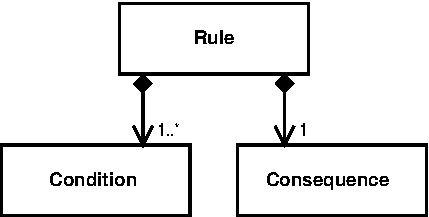
\includegraphics{rule}
  \end{center}
  \caption{Object model for \class{Rule}, \class{Condition} and \class{Consequence}}
\end{figure}

\subsection{\indexClass{RuleSet}}

A \indexClass{RuleSet} is simply a collection of \indexClass{Rule}s.
It serves only to associate a group of rules with one another so that
they may be worked with as a set.

\begin{figure}
  \begin{center}
  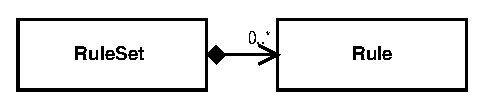
\includegraphics{ruleset}
  \end{center}
  \caption{Object model for \class{RuleSet} and \class{Rule}}
\end{figure}

\subsection{\indexClass{RuleBase}}

A \indexClass{RuleBase} is an \emph{active} collection of
\indexClass{RuleSet}s.  A \indexClass{RuleBase} contains rules
that are all considered to be in effect for a given set of
knowledge.  Multiple \class{RuleSet}s may be a part of a 
given \class{RuleBase}.

\begin{figure}
  \begin{center}
  
\includegraphics{rulebase}
  \end{center}
  \caption{Object model for \class{RuleBase} and \class{RuleSet}}
\end{figure}

\section{Knowledge}

The set of knowledge that is examined is modelled by the class
\indexClass{WorkingMemory}, which is backed by a particular
\indexClass{RuleBase}.  It is through the \indexClass{WorkingMemory}
that knowledge is \emph{asserted}, \emph{retracted} and
\emph{modified}.
Each \class{WorkingMemory} is backed by exactly one
\indexClass{RuleBase} which determines which rules are evaluated
as knowledge is manipulated.

\begin{figure}
  \begin{center}
  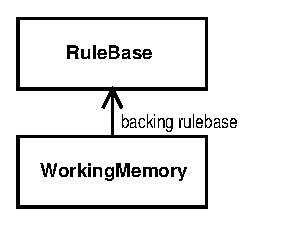
\includegraphics{workingmemory}
  \end{center}
  \caption{Object model for \class{WorkingMemory} and \class{RuleBase}}
\end{figure}

\clearpage

\section{Complete Model}

\begin{figure}[h]
  \begin{center}
  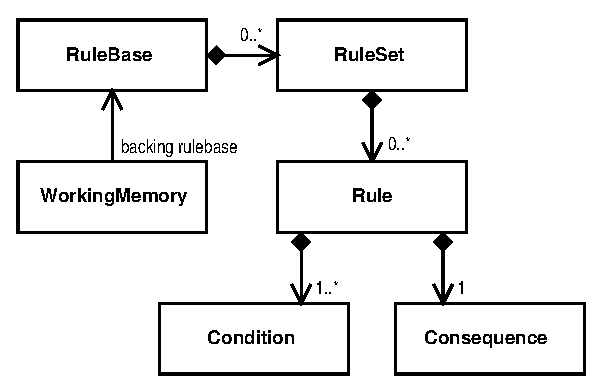
\includegraphics{architecture}
  \end{center}
  \caption{Complete object model}
\end{figure}

\chapter{Semantics Management Framework}

\dots not implemented yet \dots

\chapter{Rule Assembly API}
\label{rule.assembly}


\part{Examples}
\chapter{Examples}

\section{Sisters and Pets}

\section{Fibonacci Calculation}

\section{Trouble-Ticket Escalation}

\section{Manners Benchmark}



\part{Appendices}
\appendix

\chapter{Algorithms}
\label{algorithms}

\section{Efficient Matching}

While it may be simple to create a rules engine that 
allows specification of business logic in a format
that is comfortable to business analysts, the matching
of the rules may still be problematic without a good
algorithm.

The rules engine must be made aware of its environment,
typically through a process called \emph{fact assertion}.
Fact assertion consists of the program asserting facts
into a rules session, or \emph{working memory}.

Whenever a fact is asserted, retracted or modified within 
the working memory, many rules may become candidates for 
firing, or may have become invalidated.  A simplistic
approach is to reevaluate all rules against the entirety
of the working memory.  This method is guaranteed to be
correct but will also certainly be sub-optimal.  Any
individual fact modification only affects a small number
of conditions in a small number of rules.  

Variations of the Rete algorithm allow the rules engine
to maintain a memory of the results of partial rule
matches across time.  Reevaluation of each condition
is no longer necessary, as the engine knows which conditions
might possibly change for each fact, and only those 
must be reevaluated.




\section{Rete\index{Rete}}
\label{algo.rete}

Charles Forgy\index{Forgy, Charles} created the original Rete algorithm\cite{forgy82rete} 
around 1982 as part
of his DARPA-funded research.  Compared to many previous
production-matching algorithms, Rete was very advanced.  Even today,
there have been few improvements to it in the general
case\footnote{Both ILOG and Haley claim to have optimized Rete
algorithms, but details are not currently public.}.  Variations on 
Rete, such as TREAT \cite{miranker87treat}, may have different performance characteristics
depending on the environment.  Some perform better with large rule 
sets but small numbers of objects, while other perform well for 
steady-state environments, but react poorly to numerous successive 
changes in the data.

A \emph{Rete network}\index{Rete!network} is a graph through which data flows.
Originally, data was specified using Cambridge-prefix tuples since
Lisp-like languages were in style for logic programming.\footnote{As it is for many artificial
intelligence projects.}  The tuples were used to express attributes
about objects.  For example, tuples may be used to express a person's
name and her pets.  The tuples are dropped into the Rete network,
and those that reach the far end cause the firing of a rule.
The original production-matching was based upon matches against
tuple patterns.

\bigskip

The Rete network is comprise of two types of nodes:

\begin{itemize}
	\item \textbf{\textsf{1-input/1-output nodes}}\\
		The \emph{1/1} nodes are
		constrictive nodes that only allow matching tuples to
		flow through.  Any tuples that do not match are discarded
		by the node.
	\item \textbf{\textsf{2-input/1-output nodes}}\\
		The \emph{2/1} nodes simply connect the output arcs from two
		other nodes (either \emph{1/1} nodes or \emph{2/1} nodes) merging
		tuples from both the left and right incoming arcs
		into a single tuple on the outgoing arc.  Maintains a memory
		of tuples for matching against future facts.
\end{itemize}

A forest of \emph{1/1} nodes acts as the entry-point
into the entire Rete network for any incoming tuple.  The
network-entry  nodes filter tuples purely by their type.  
Tuples about dogs and tuples about cats may 
each have a different type and may be differentiated from each 
other by the \emph{1/1} network-entry nodes.

Each condition of a rule is merely a pattern for a particular tuple type.
The condition describes the attributes that a tuple must have and acts
as a filter.  Each condition is transformed into a \emph{1/1} node
that only allows tuples matching the specified attributes to pass.
An attribute value may be specified as a variable and implies that
the variable must hold the same value in all occurrences.
The \emph{1/1} filter nodes are attached to
the network downstream from the \emph{1/1} entry-node that
differentiates their tuple type.

Consider a condition such as ``For any person who has a dog that
has the same name as that person's sister's cat, then...''  This could
be expressed with the condition patterns of:

\medskip

\begin{tabular}{llll}

(1) & \texttt{( person} & \texttt{name=person?} & \texttt{sister=sister? )}\\
(2) & \texttt{( person} & \texttt{name=person?} & \texttt{dog=petName? )}\\
(3) & \texttt{( person} & \texttt{name=sister?} & \texttt{cat=petName? )}\\

\end{tabular}

\medskip

Condition \emph{\#1} models the sister relationship so
that the rule only applies to two people who are sisters.  The
\verb|person?| and \verb|sister?| tokens are variables that must be
consistent across any set of tuples that match this rule.  

Conditions \emph{\#2} and \emph{\#3} serve two roles.  The \verb|dog|
and \verb|cat| attributes share the same \verb|petName?| variable and
serve to identify two people who have a cat and a dog with the same
name.  They each contain a \verb|name| attribute with either the
variable \verb|person?| or \verb|sister?| which ties the last two
conditions back to the first two.

\begin{figure}[htbpc]
  \begin{center}
   \begin{minipage}{6in}
	\xymatrix {
		\bullet \ar[d] \\
		type(person) \ar[d] \ar[dr] \ar[drr] \\
%
	condition(1) \ar[dr] & condition(2) \ar[d] & condition(3) \ar[dd] \\
%
	       & join(1) \ar[dr] \\
%
	       & & join(2) \ar[d] \\
%
	       & & terminal \\
	}
  \end{minipage}
  \end{center}
  \label{network.rete}
  \caption{Rete network}
\end{figure}

\setlength{\extrarowheight}{3pt}


\begin{figure}[htbpc]
  \begin{center}
    \begin{tabular}{|c||c|c|c|c|}
      \hline
        \emph{\textsf{type}} %
            & \textsf{person} %
            & \textsf{sister} %
            & \textsf{cat} %
            & \textsf{dog} \\
      \hline
      \hline
        \multicolumn{5}{|c|}{\emph{tuple set \# 1}}\\
      \hline 
      \hline 
        person & rebecca & jeannie & zoomie & \emph{null} \\
      \hline
        person & jeannie & rebecca & \emph{null} & zoomie \\
      \hline
      \hline
        \multicolumn{5}{|c|}{\emph{tuple set \# 2}}\\
      \hline
      \hline
        person & rebecca & jeannie & zoomie & \emph{null} \\
      \hline
        person & jeannie & rebecca & \emph{null} & toby \\
      \hline
    \end{tabular}
  \end{center}

  \caption{Example tuple sets}
  \label{table.tuplesets}
\end{figure}

\clearpage

If two sets of tuples (see Figure \ref{table.tuplesets}) were
asserted against the rule, \emph{tuple set \#1} would cause a firing
of the rule, where \emph{tuple set \#2} would not.  In both cases,
the two tuples would pass node \emph{condition(1)}, as the
nodes simply associate the \verb|person?| and \verb|sister?| variables
with the appropriate values from each tuple.

The \emph{join(1)} node would allow both tuples to merge and
propagate past it in both the first and second case.  Additionally,
for both cases, the \emph{rebecca} tuple would pass node
\emph{condition(2)}
and the \emph{jeannie} tuple would pass node \emph{condition(3)}.

The \emph{join(2)} node is where the two cases differ.  In the first
case, nodes \emph{condition(2)} and \emph{condition(3)} have each associated the value
of ``ugly'' to the \verb|petName?| variable.  In the second case, the
two nodes has assigned different values to the variable.  The
\emph{join(2)} node only allows those tuples that have consistent
associations with all variables to pass.


\section{Rete-OO}

The Rete algorithm works wonderfully in language systems 
such as Lisp where pertinent attributes about objects 
are directly asserted to the rules engine.  In an
object-oriented language, such as C++ or Java, and entire 
graph of objects can be reachable from a single named 
root object.  Expressing highly complex relationships between
entities using Cambridge-prefix notation may require many
separate assertions.  In an OO language, the single root
object is all that should be asserted, since attributes 
and relationships can be \emph{extracted} using normal
language constructs.

Bob McWhirter of The Werken Company adapted Forgy's original Rete 
algorithm to object-oriented constructs, creating the Rete-OO algorithm.
As with Rete, there are \emph{1/1} nodes and \emph{2/1}
nodes.  Unlike Rete, there are nodes that exist simply 
to extract reachable attributes and add columns to passing
tuples. Rete always constructs the condition \emph{1/1} nodes toward
the root of the tree leaving the bottom portion to be 
comprised of purely aggregating \emph{2/1} \emph{join} nodes.  
Rete-OO must interleave both \emph{1/1} and \emph{2/1} nodes.

The same example as in section \ref{algo.rete}, 
the conditions could be expressed in terms of object-oriented
language boolean and assignment expressions.  The choice
of Java as the expression language is purely arbitrary.

\medskip

\begin{tabular}{cl}
(0) & \texttt{Person personOne, personTwo} \\
(1) & \texttt{personOne.hasSister(personTwo)} \\
(3) & \texttt{petName = personOne.getCat().getName()} \\
(3) & \texttt{petName = personTwo.getDog().getName()} \\
\end{tabular}

\bigskip

Rete-OO adds the concept of \emph{root object declaration}, where 
the root objects of the condition are declared with a
name and type.  The object's type maps directly to the
tuple type in Rete.  The root object name has no direct
mapping in Rete and causes the addition of a \emph{parameter node}
in Rete-OO.  Boolean expressions in Rete-OO conditions are
equivalent to Rete's condition patterns against attributes.
The assignment expressions map to place-holder variables in
Forgy's algorithm.

The types of nodes used in Rete-OO graph construction are
listed here.  Those that are new or different from Rete are
denoted with a '*'.

\begin{itemize}
	\item \textsf{\textbf{Object type}} \\
		Object type nodes differentiate objects by
		filtering on their defined type.
	\item \textsf{\textbf{Parameter*}}\\
		Parameter nodes create a tuple with a single
		entry binding the object to the name.
	\item \textsf{\textbf{Condition}}\\
		Condition nodes simply tests a tuple against 
		an a boolean expression.
	\item \textsf{\textbf{Extraction*}}\\
		Extraction nodes extract new attributes, 
		create new columns on tuples, and store the
		results.
	\item \textsf{\textbf{Join}}\\
		Join nodes connect the output arcs from two
		other nodes and allows consistent tuples to
		be merged and passed through.
	\item \textsf{\textbf{Terminal}}\\
		Terminal nodes fire to indicate a successful
		match for the rule.  
\end{itemize}

The resulting Rete-OO graph is constructed in a different
manner than the equivalent Rete graph, due to the addition
and rearrangement of some nodes.

\begin{figure}
\begin{center}
  \begin{minipage}{6in}
	\xymatrix @R-10pt{
		\bullet \ar[d] \\
		type(Person) \ar[d] \ar[dr] \\
		parameter(personOne) \ar[d] & parameter(personTwo) \ar[d] \\
		extraction(petName) \ar[dr] & extraction(petName) \ar[d] \\
		 & join \ar[d] \\
		 & condition(hasSister) \ar[d] \\
		 & terminal \\
	}
  \end{minipage}
\end{center}
\label{network.rete-oo}
\caption{Rete-OO network}
\end{figure}



\chapter{Frequently Asked Questions}\index{FAQ|see Frequently Asked
Questions}\index{Frequently Asked Questions}
\label{faq}

\section{Why are ``or'' conditions not allowed?}

\section{Can I nest rules?}

\section{What happened to version 1.0?}

\chapter{Project Information}


\section{Web Site}

All development resources related to Drools are hosted by 
\textbf{The Codehaus}\index{Codehaus, The}, the open-source 
arm of The Werken Company. Drools maintains a website at:

\begin{quote}
	\url{http://drools.org/}
\end{quote}


\section{Mailing Lists}

The drools project maintains two mailing lists.  The first, known as
\verb|user| is for general discussion by users and
developers of drools.  The second list is \verb|scm| which
simply tracks changes made to the source-code through the CVS
repository. For information about subscribing to each list or access 
to the list archives:

\begin{quote}
    \url{http://archive.drools.codehaus.org/user/}\\
    \url{http://archive.drools.codehaus.org/scm/}
\end{quote}

\section{Source Repository}

The drools project maintains a revision control repository using
CVS.  To checkout the latest sources, you must issue two CVS commands.
The first is used to login.  When presented with a prompt for a
password, simply press \emph{ENTER}.

{\small
\begin{verbatim}
  cvs -d:pserver:anonymous@cvs.drools.codehaus.org:/home/projects/drools/scm login
  cvs -d:pserver:anonymous@cvs.drools.codehaus.org:/home/projects/drools/scm co drools
\end{verbatim}
}

\clearpage

\section{Internet Relay Chat}

There is a dedicated channel on The Werken Company's IRC server for
drools:\\

\begin{tabular}{rl}
address & \verb|irc.codehaus.org| \\
port    & \verb|6667| \\
channel & \verb|#drools|\\
url     & \url{irc://irc.codehaus.org:6667/drools}\\
\end{tabular}

\bigskip

\section{Bug, Issue \& Feature Tracking}

For bug, issue and feature tracking, the Drools project uses the
Jira project management system provided by The Codehaus.

\begin{quote}
    \url{http://jira.codehaus.org/}
\end{quote}

\clearpage

\section{Project Team}

\subsection{Bob McWhirter\index{McWhirter, Bob}}

Bob McWhirter originally founded the Drools project in 2000 and
developed the Rete-OO algorithm used by the engine.  Bob is also
the founder of The Werken Company and the chief architect behind
the commercial \textbf{Fluxtapose} suite of tools which build
upon Drools to provide a complete solution for implementing
business rules.

\subsection{Thomas Diesler\index{Diesler, Thomas}}

Thomas Diesler researched and supplied the JSR-94 Rule-Engine API
bindings for Drools.

\begin{ednote}
Thomas, please send more details to \texttt{bob@werken.com}.
\end{ednote}

\subsection{Roger F. Gay\index{Gay, Roger F.}}

Roger F. Gay devised the XML Schemas for the core DRL syntax and
each semantic module.

\begin{ednote}
Likewise, Roger, please send more details to \texttt{bob@werken.com}.
\end{ednote}

\subsection{Contributors}

Others have contributed ideas, patches and testing assistance
over the years:

\begin{itemize}
  \item Dave Cramer\index{Cramer, Dave} \emph{(eBox)}
  \item Martin Hald\index{Hald, Martin}
  \item Matt Ho\index{Ho, Matt}
  \item Pete Kazmier\index{Kazmier, Pete} \emph{(iBasis)}
  \item Christiaan ten Klooster\index{Klooster, Christiaan ten}
  \item James Roome\index{Roome, James}
  \item Bart Selders\index{Selders, Bart} \emph{(iBanx)}
  \item James Strachan\index{Strachan, James} \emph{(Core Developers Network)}
  \item Tom Vasak\index{Vasak, Tom}
\end{itemize}


\begin{ednote}
Hello to contributors: send your current affiliation information
to \texttt{bob@werken.com} if you wish it to be included.
\end{ednote}


\chapter{Licensing}

\section{\drools{} License}

\subsection{The License}

\small

{\center \textbf{\textsf{Copyright 2002 (C) The Werken Company. All Rights Reserved.}}\\}

\bigskip

Redistribution and use of this software and associated documentation
(``Software''), with or without modification, are permitted provided
that the following conditions are met:

\begin{enumerate}
	\item Redistributions of source code must retain copyright
   statements and notices.  Redistributions must also contain a
   copy of this document.
 
	\item Redistributions in binary form must reproduce the
   above copyright notice, this list of conditions and the
   following disclaimer in the documentation and/or other
   materials provided with the distribution.
 
	\item The name \drools{} must not be used to endorse or promote
   products derived from this Software without prior written
   permission of The Werken Company.  For written permission,
   please contact info@werken.com.
 
	\item Products derived from this Software may not be called \drools{}
   nor may \drools{} appear in their names without prior written
   permission of The Werken Company. \drools{} is a registered
   trademark of The Werken Company.
 
	\item Due credit should be given to The Werken Company. 
\end{enumerate}
 
THIS SOFTWARE IS PROVIDED BY THE WERKEN COMPANY AND CONTRIBUTORS
\textbf{AS IS} AND ANY EXPRESSED OR IMPLIED WARRANTIES, INCLUDING, BUT
NOT LIMITED TO, THE IMPLIED WARRANTIES OF MERCHANTABILITY AND
FITNESS FOR A PARTICULAR PURPOSE ARE DISCLAIMED.  IN NO EVENT SHALL
THE WERKEN COMPANY OR ITS CONTRIBUTORS BE LIABLE FOR ANY DIRECT,
INDIRECT, INCIDENTAL, SPECIAL, EXEMPLARY, OR CONSEQUENTIAL DAMAGES
(INCLUDING, BUT NOT LIMITED TO, PROCUREMENT OF SUBSTITUTE GOODS OR
SERVICES; LOSS OF USE, DATA, OR PROFITS; OR BUSINESS INTERRUPTION)
HOWEVER CAUSED AND ON ANY THEORY OF LIABILITY, WHETHER IN CONTRACT,
STRICT LIABILITY, OR TORT (INCLUDING NEGLIGENCE OR OTHERWISE)
ARISING IN ANY WAY OUT OF THE USE OF THIS SOFTWARE, EVEN IF ADVISED
OF THE POSSIBILITY OF SUCH DAMAGE.

\normalsize

\subsection{Summary}

\drools{} is provided under a license similar to that used by
The Apache Software Foundation.  It is a commercial-friendly license
in that it allows you to modify and distribute \drools{} in either
source or binary form.  While you are \emph{encouraged} to contribute
changes back to the project, you are by no means \emph{required} to
do so.   The \drools{} license is not viral or infectious.  It
does not alter how you license you own product.  If you have any
questions regarding the licensing of \drools{}, please contact
\verb|info@werken.com|.

\clearpage

\section{3rd-Party Licenses}

\drools{} contains software written by The Werken Company and by
other third-party groups.  Included are the licenses of included
components.


\subsection{Apache Jakarta}

\small

The Apache Software License, Version 1.1

{\center \textbf{\textsf{Copyright (c) 2001 The Apache Software Foundation.  All rights reserved.}}\\}

\bigskip

Redistribution and use in source and binary forms, with or without
modification, are permitted provided that the following conditions
are met:

\begin{enumerate}
	\item Redistributions of source code must retain the above copyright
		notice, this list of conditions and the following disclaimer.

	\item Redistributions in binary form must reproduce the above copyright
		notice, this list of conditions and the following disclaimer in
		the documentation and/or other materials provided with the
		distribution.

	\item The end-user documentation included with the redistribution,
		if any, must include the following acknowledgment:
		``This product includes software developed by the
		Apache Software Foundation (http://www.apache.org/).''
		Alternately, this acknowledgment may appear in the software itself,
		if and wherever such third-party acknowledgments normally appear.

	\item The names ``Apache'' and ``Apache Software Foundation'' 
		must not be used to endorse or promote products
		derived from this software without prior written permission. For
		written permission, please contact apache@apache.org.

	\item Products derived from this software may not be called
	``Apache'', nor may ``Apache'' appear in their name, without
	prior written permission of the Apache Software Foundation.
\end{enumerate}

THIS SOFTWARE IS PROVIDED \textbf{AS IS} AND ANY EXPRESSED OR IMPLIED
WARRANTIES, INCLUDING, BUT NOT LIMITED TO, THE IMPLIED WARRANTIES
OF MERCHANTABILITY AND FITNESS FOR A PARTICULAR PURPOSE ARE
DISCLAIMED.  IN NO EVENT SHALL THE APACHE SOFTWARE FOUNDATION OR
ITS CONTRIBUTORS BE LIABLE FOR ANY DIRECT, INDIRECT, INCIDENTAL,
SPECIAL, EXEMPLARY, OR CONSEQUENTIAL DAMAGES (INCLUDING, BUT NOT
LIMITED TO, PROCUREMENT OF SUBSTITUTE GOODS OR SERVICES; LOSS OF
USE, DATA, OR PROFITS; OR BUSINESS INTERRUPTION) HOWEVER CAUSED AND
ON ANY THEORY OF LIABILITY, WHETHER IN CONTRACT, STRICT LIABILITY,
OR TORT (INCLUDING NEGLIGENCE OR OTHERWISE) ARISING IN ANY WAY OUT
OF THE USE OF THIS SOFTWARE, EVEN IF ADVISED OF THE POSSIBILITY OF
SUCH DAMAGE.

\normalsize

\clearpage

\subsection{Beanshell}

\small

{\center \textbf{\textsf{Copyright (C) 2002 The Beanshell Project}}\\}

\bigskip

This library is free software; you can redistribute it and/or
modify it under the terms of the GNU Lesser General Public
License as published by the Free Software Foundation; either
version 2.1 of the License, or (at your option) any later version.

This library is distributed in the hope that it will be useful,
but WITHOUT ANY WARRANTY; without even the implied warranty of
MERCHANTABILITY or FITNESS FOR A PARTICULAR PURPOSE.  See the GNU
Lesser General Public License for more details.

You should have received a copy of the GNU Lesser General Public
License along with this library; if not, write to the Free Software
Foundation, Inc., 59 Temple Place, Suite 330, Boston, MA  02111-1307  USA

\normalsize

\subsection{ANTLR}

\small

SOFTWARE RIGHTS

{\center \textbf{\textsf{ANTLR 1989-2000 Developed by jGuru.com,
(MageLang Institute), \\ 
http://www.ANTLR.org  and http://www.jGuru.com}}\\}

\bigskip

We reserve no legal rights to the ANTLR--it is fully in the
public domain. An individual or company may do whatever
they wish with source code distributed with ANTLR or the
code generated by ANTLR, including the incorporation of
ANTLR, or its output, into commerical software.

We encourage users to develop software with ANTLR. However,
we do ask that credit is given to us for developing
ANTLR. By "credit", we mean that if you use ANTLR or
incorporate any source code into one of your programs
(commercial product, research project, or otherwise) that
you acknowledge this fact somewhere in the documentation,
research report, etc... If you like ANTLR and have
developed a nice tool with the output, please mention that
you developed it using ANTLR. In addition, we ask that the
headers remain intact in our source code. As long as these
guidelines are kept, we expect to continue enhancing this
system and expect to make other tools available as they are
completed.

\normalsize


\backmatter

\bibliography{manual}
\bibliographystyle{acm}

{\footnotesize
\pagestyle{plain}
\printindex
}

%\pagestyle{plain}

\rule{0pt}{17em}

\begin{center}
\begin{minipage}{0.6\textwidth}
\noindent
This manual was produced without the aid of Microsoft products.
It was authored on a Linux laptop using XEmacs\index{XEmacs} and
\LaTeX\index{Latex@\LaTeX}.  Drafts were previewed using
\texttt{xdvi}. Diagrams were prepared using \texttt{dia}, exported
in EPS format and converted for inclusion in the PDF document with \texttt{epstopdf}.  
The index was prepared using the \texttt{makeindex} package.
\end{minipage}
\end{center}



\end{document}
